\documentclass[12pt]{article}
\usepackage{hyperref}
\usepackage{natbib}
\usepackage{amsmath}
\usepackage{nicefrac}
\usepackage[usenames,dvipsnames]{xcolor}
\usepackage{graphicx}
\usepackage{footnote}
\usepackage{rotating}
%\usepackage{slashbox}
\usepackage{afterpage}
\usepackage{float}
\usepackage{color}
\usepackage{array}

\usepackage[margin = 1.0 in]{geometry}
%\bibliographystyle{ynt}
\usepackage{natbib}
%\usepackage[natbib=true,style=numeric,sorting=ynt]{biblatex}


\renewcommand{\bottomfraction}{.9}
\renewcommand{\topfraction}{.9}
\renewcommand{\textfraction}{0.1}
\renewcommand{\floatpagefraction}{.9}


%%%%%%%%%%%%%%%%%%%%%%%%%%%%%%%%%%%%%%%%%%%%%%%%%%%%%%%%%%%%%%%%%%%%%%%%%%%%
%   document style macros
%%%%%%%%%%%%%%%%%%%%%%%%%%%%%%%%%%%%%%%%%%%%%%%%%%%%%%%%%%%%%%%%%%%%%%%%%%%%
\def\gtrsim{\mathrel{\hbox{\rlap{\hbox{\lower4pt\hbox{$\sim$}}}\hbox{$>$}}}}
\def\lessim{\mathrel{\hbox{\rlap{\hbox{\lower4pt\hbox{$\sim$}}}\hbox{$<$}}}}
\newcommand{\ddg}{$\Delta\Delta G~$}
%%%%%%%%%%%%%%%%%%%%%%%%%%%%%%%%%%%%%%%%%%%%%%%%%%%%%%%%%%%%%%%%%%%%%%%%%%%%

\graphicspath{{../figures/}}

\title{Variation in site entropy explains differences in structure-sequence relationships of proteins}
\author{Eleisha L. Jackson$^{1^*}$, Amir Shahmoradi$^{1*}$, Claus O. Wilke$^{1^{**}}$}
\begin{document}

\date{\today}
\maketitle


\noindent
%$^1$ Department of Physics, The University of Texas at Austin, Austin, TX 78712, USA \\
$^1$ Institute of Cellular and Molecular Biology, Center for Computational Biology and Bioinformatics, and Department of Integrative Biology, The University of Texas at Austin, Austin, Texas, 78712 USA\\

\noindent $^{*}$These authors contributed equally. \\

\bigskip
\noindent
$^{**}$Corresponding author\\
%$\phantom{^*}$Email: amir@physics.utexas.edu\\
$\phantom{^{** }}$Email: wilke@austin.utexas.edu\\
%$\phantom{^*}$Phone:{ \color{red} Need a phone} \\
$\phantom{^{**}}$Phone: +1 512 232 2459\\

\bigskip
\noindent
Manuscript type: research article\\
\bigskip
\noindent  Keywords: protein evolution, relative solvent accessibility, site variability


\begin{abstract}
Recent work has shown that structural properties are capable of predicting site-specific sequence variability for a given protein. However, the strength and significance of these structure-sequence relations appear to vary widely among different proteins, with absolute correlation strengths ranging from $0.1$ to $0.8$. There have two works that have investigated structural predictors of site variability which both present different results based on the strength of correlations of structural predictors. According to \cite{Yehetal2014a}, both solvent accessibility and local packing density are predictors of site-wise variability with local packing density being strongest predictor of site-wise variability. However, recently, \cite{Shahmoradietal2014} compared local packing density, residue flexibility, and solvent accessibility in viral proteins and found that relative solvent accessibility is a stronger predictor of site-wise variability. In addition, the strength of correlations with structural predictors were weaker in \cite{Shahmoradietal2014}.  Here we present research that suggests that differences in the correlations between these two datasets are due to differences in the site variability among proteins within in each dataset. Specifically proteins with a larger variance in entropy among sites exhibit stronger structure-sequence correlations between both local packing density and solvent accessibility. 
\end{abstract}
\vfill
\vfill
\def\thefootnote{\fnsymbol{footnote}}
\setcounter{footnote}{0}


\section{Introduction}
\label{sec:intro}

The effect of protein-protein interactions(Fraser 2002)

Proteins are subject to a number of biophysical and functional constraints \citep{Scherreretal2012, Wilkeetal2010, Sikoseketal2014, Liberlesetal2009, Huangetal2014, Fraseretal2002, Liaoetal2010, Serohijosetal2012}. These constraints result in site-specific patterns of sequence variability within a protein. Recently several site-specific structural properties that can explain patterns of sequence variability in proteins have been identified. One of the earliest examples was Relative Site Accessibility (RSA). \cite{Fransozaetal2009} identified RSA as the strongest predictor of evolutionary rate and found that residues that are buried within the core of proteins tend to be more conserved than exposed residues close to the surface of the protein. In their analysis, they considered the ability of both RSA and various definitions of residue packing density to predict evolutionary rate. They found that RSA and evolutionary rate shared a significant linear relationship. Afterwards, several other works  also found that RSA as a significant predictor of evolutionary rate and supported this linear relationship \citep{Ramseyetal2011, Scherreretal2012}. However, these papers all have the same flaw. During the course of their analysis they binned the protein sites and averaged over all sites within a bin when determining the trend of RSA. This process may have produced artifacts that account for this strong linear trend between RSA and evolutionary rate. \\
\indent Recently, \cite{Yehetal2014a} performed a similar analysis on a series of enzyme monomer proteins and found that packing density, as defined by Contact Number and Weighted Contact Number \citep{Liaoetal2005, Yehetal2014a, Huangetal2014}, was the strongest determinant of site variability.  Soon Afterwards, \cite{Shahmoradietal2014} also performed a site-wise analysis on a series of viral proteins. In this analysis they found that RSA had a slightly stronger correlation with site variability as opposed to local packing density.  Moreover, the effect seen between CN and WCN was of a much smaller magnitude as compared to \cite{Yehetal2014a}. It is not well understood the reasoning behind the difference in magnitude in the correlations seen between the two studies. Here we attempt to reconcile the work done in this area. We find that site variability is the primary determinant of the strength of structure-sequence relationships and some differences in previous work can be explained in terms of differing levels of site variability. \\

\section{Materials and Methods}
\label{sec:mam}

    \subsection*{Structures, sequences, and measures of sequence properties } 
    The results presented in this work are based on two datasets. The first is a dataset of $209$ monomeric enzymes taken from \cite{Huangetal2014}, originally from \cite{Yehetal2014a}.The original dataset was comprised of $213$ proteins but we removed four of the proteins (PDB IDS: 1BBS, 1BS0, 1DIN, 2HPL) that had did not have data at insertion sites. Briefly, these proteins are all enzyme monomers   randomly picked from the Catalytic Site Atlas $2.2.11$ \citep{Porteretal2004} with protein sizes in the sample ranging from $95$ to $1287$ residues in length. For each structure we had a corresponding alignment of up to 300 homologous sequences.  The second dataset was taken from \cite{Shahmoradietal2014} and is comprised of nine viral proteins. The viral proteins range from 122 - 557 residues in length and each structure is accompanied by a sequence alignment of up to 2362 homologous sequences. Sequence alignments for both datasets were constructed by aligning the amino-acid sequences using the alignment software MAFFT \citep{Katohetal2002, Katohetal2005}, specifying the auto flag to select the optimal algorithm for the given dataset. The alignments were then used to calculate site-specific measures of sequence variability for each individual protein in both datasets. To do so, we relied on two independent methods of measuring sequence variability. First, we calculated the Shannon entropy ($H_i$) -- the sequence entropy at each alignment column $i$:
    \begin{equation}
        \label{eqn:shannon}
        H_i = -\sum_j P_{ij}\ln P_{ij}
    \end{equation}

    where $P_{ij}$ is the relative frequency of amino acid $j$ at position $i$ in the alignment. Sequence entropy is a measure of variability at each site. We also calculated a measure of site-specific evolutionary rate for each protein using the software Rate4site. First Maximum Likelihood phylogenetic trees were inferred with RAxML, using the LG substitution matrix and the CAT model of rate heterogeneity \citep{Stamatakis2006, Stamatakis2014}. For each structure, we then used the respective sequence alignment and phylogenetic tree to infer site-specific substitution rates with Rate4Site using the empirical Bayesian method and the JTT model of sequence evolution \citep{Mayroseetal2004}.

    \subsection*{Calculation of Structural Properties}
In our analysis we used two types of measures of local packing density used in previous studies: Contact Number (CN) and Weighted Contact Number (WCN). For the purposes of our comparison between the two datasets of interest we used the CN and WCN for the enzyme proteins calculated in \cite{Huangetal2014} and the CN and WCN values for the viral proteins from \cite{Shahmoradietal2014}. In both of these works and in \cite{Yehetal2014a}, WCN and CN are both defined the same.  Contact Number is defined as the number of $C_{\alpha}$ within a pre-redefined radius, $r_0$. In this case, $r_0$ = 13 as in the previous papers. Weighed Contact Number for a residue, $i$, is defined as in \cite{Liaoetal2005} and \cite{Huangetal2014} as:
	
	\begin{equation} \label{wcn_eqn}
		\text{WCN}_i = \sum_{i \neq j}^{N} \frac{1}{r_{ij}^2 } 
	\end{equation}
	
	where $r_j$ is the length between the $C_{\alpha}$ of residue $i$ and residue $j$ in a protein of length $N$ \citep{Yehetal2014a}. 

\indent We used DSSP \citep{Kabschetal2005} to calculate the Accessible Surface Area (ASA) for each site. We then normalized the ASA for each site by the theoretical maximum solvent accessibility values of \cite{Tienetal2013} to obtain the Relative Solvent Accessibility (RSA) for all individual sites in all proteins. \\

All data and analysis scripts required to reproduce the work are publicly available to view and download at \url{https://github.com/wilkelab/rate_variability_variation}.

\section{Results}
\label{sec:results}

Although it is clear that structure plays a role in the evolution of proteins, it is not clear to what extent protein structure constrains sequence variability. To date there have been conflicting reports about the strength of structure-sequence correlations \citep{Yehetal2014b, Shahmoradietal2014}. Therefore we sought to determine the main determinants of structure-sequence correlations within proteins. First, we calculated the strength between the structural properties and site variability by calculating the Spearman correlation, $\rho$,  between the structural property (solvent exposure and local packing density) and site variability, as measured by either evolutionary rate or site entropy. On average the correlations between CN and entropy are larger in absolute magnitude in the enzyme proteins as compared to viral proteins. The average $\rho$ between each structural property and each measure of site variability (entropy and evolutionary rates) can be seen in Table \ref{table:entropy_stats}  and Table \ref{table:rate_stats}. The viral proteins experience much lower site variability. Figure 1 shows the correlations between CN and entropy for the viral and enzyme proteins. Even though on average the correlations in the enzyme proteins are larger as reported by \cite{Yehetal2014a}, the viral proteins still have correlation strengths that are comparable to some of the enzyme proteins with lower correlations. 

\indent For a given protein its mean entropy and the variance might be different. A protein can have a high mean entropy but have a low variance and vice versa. Figure \ref{fig:protein_ex_plot}A details the relationship between the average entropy across sites within proteins and the variance of entropy across sites. Additionally, the distribution of variance varies greatly between proteins even when they from the same dataset (Figure \ref{fig:protein_ex_plot}B). Therefore the mean entropy of a protein as well as the variance in entropy at sites may be predictive for structure-sequence relationships.

\indent  The average site entropy of a given protein does not seem to be a significant determinant of the strength of structural correlations (Figures \ref{fig:entropy_cn_cor}A, \ref{fig:entropy_wcn_cor}A, \ref{fig:entropy_rsa_cor}A). However, when examining the variance of entropy there is a clear trend within the enzyme proteins.  Proteins with a higher variance in site variability across the protein typically higher  correlations in magnitude (Figures \ref{fig:entropy_cn_cor}B, \ref{fig:entropy_wcn_cor}B, \ref{fig:entropy_rsa_cor}B). If you extrapolate the trend from the enzyme proteins, the viral proteins follow a similar trend. The correlation between the $\rho$ between RSA and entropy and the variance of entropy is positive. Proteins with a larger variance in site entropy have the strongest correlations. The correlation between local packing density (both WCN and CN) and the variance of entropy is negative. Unlike entropy, there is no relationship between the variance of evolutionary rates at sites and any of the measured structural properties (Figures \ref{fig:var_rate_cor}, \ref{fig:var_rate_rsa_cor}). There also is a wide spread in the variance of the evolutionary rates across proteins for both the enzyme and viral proteins. 

\indent Although both evolutionary rate, as measured by Rate4Site and entropy are measures of site variability, these quantities are distinctly different. Rate4Site measures the rate at which a site changes over time whereas site entropy measure the absolute variation at a site. A site may have a high evolutionary rate if it changes  frequently between the same few amino acids but have low entropy. It appears that the rate at which a site evolves is not important for predicting the strength of structure-sequence relationships. However, the absolute amount of variation at a site can be used to predict the strength of structure-sequence relationships. 

\indent In order to further examine the relationship between entropy and the structure-sequence relationships, we used the mean entropy and variance of entropy at sites as predictors of the strength of structure-sequence relationships. Table \ref{table:model_stats} illustrates the coefficients of various linear models. For WCN-Entropy correlations, mean entropy is not a significant predictor. Although for CN-Entropy correlations, mean entropy is significant the coefficient is 0.079 and therefore predictive power is low. Mean Entropy is also not a significant predictor for the strength of the relationship between RSA and Entropy. For all linear models where mean entropy and dataset were used to predict structure-sequence correlations, dataset was a significant predictor (Table \ref{table:model_stats}). This means that enzyme and virus proteins have different correlations when using mean entropy as a predictor. This agrees with differences seen in the previous works by \cite{Yehetal2014a} and \cite{Shahmoradietal2014}.  

\indent However, when looking at the variance in entropy there are some stark differences. For all structural predictors (i.e., CN, WCN and RSA), the variance in entropy at sites within a protein is a significant predictor of the strength of structure-sequence relations. For packing density, proteins with a larger variance in site-wise entropy have more negative correlations that are higher in magnitude. Proteins with a higher variance in entropy tend to have stronger RSA-Entropy correlations. When using variance and dataset as predictors of structure-sequence correlations, dataset was not a significant predictor in any model. When looking at the variance of entropy, proteins within both datasets at in a similar fashion and overall trends seen between the variance of site variation and the strength of structure-sequence relationships is preserved across both datasets. 

\section{Discussion}
\label{sec:dcr}

There has been previous work that has illuminated several factors that determine the rate at which proteins evolve \citep{Fraseretal2002, Drummondetal2008, Wilkeetal2010, Yangetal2012}. Some of these factors include: expression level \citep{Drummondetal2008, Wilkeetal2010, Paletal2001, Subramanianetal2004}, interactions with other protein partners \citep{Fraseretal2002, Yangetal2012, Minterisetal2005, Pangetal2010}  and selection for the costs of misfolding \citep{Drummondetal2005}. 

\indent Proteins are under a number of constraints for function \citep{Liberlesetal2009}. Biophysical considerations that have been shown to affect function include: selection for protein stability and proper folding \citep{Drummondetal2005}, specificity for protein binding \citep{Zarrinparetal2003}  and selection against non-specific and extraneous binding \citep{Levyetal2012}, selection to minimize protein aggregation \citep{DePristoetal2005}  and protein structure \citep{Fransozaetal2009, Fransozaetal2012, Yehetal2014a, Yehetal2014b, Shahmoradietal2014, Echaveetal2015, Huangetal2014}. Recently there have been several works that have looked into the effect of protein structure on protein function. Local packing density and solvent accessibility have been emerged as two structural predictors that have been showed to predict site variability \citep{Yehetal2014a, Yehetal2014b, Shahmoradietal2014, Fransozaetal2009, Bustamanteetal2000}. 

\indent Structure imposes constraints on the evolution of proteins. Therefore structural predictors can be used to predict the variability at sites. Two main determinants of variability at protein sites are solvent accessibility and local packing density. Sites that are on surface of the protein tend to have higher solvent accessibility and exhibit more site variability. Sites that are densely packed and have more contacts tend to evolve slower and exhibit less sequence variability. However, the strength of how well these two structural quantities (local packing density and solvent accessibility) has not been clearly explained. \cite{Yehetal2014a} examined the effect of using solvent accessibility and local packing density as measures of predicting site-wise variability. They found that both were predictors. However, \cite{Shahmoradietal2014} performed the same analysis on viral proteins and found that will both were predictors of stir-wise variability, the correlations between these two structural predictors and site variability were significantly lower. 

\indent Here we examined the relationship between site variability and the strength of structure-sequence relationships in order to dissect the nature of the correlation between structural properties and site variability. We found that proteins with a larger variance in site variability as measured by sequence entropy, have stronger structure-sequence relationships on average. However, when looking at the mean entropy values of proteins there is a distinct difference between the virus and enzyme datasets. Overall the enzyme proteins have more site variability than the viral proteins. When predicting structure-sequence relationships the variance in site variability among proteins is a better predictor than mean site variability.  \indent Additionally the reason that the enzyme proteins in \cite{Yehetal2014a} had higher correlation coefficients is that on average, the enzyme proteins have larger variance in entropy as compared to the virus proteins of \cite{Shahmoradietal2014}. Moreover, since the variance in entropy is a more significant predictor of correlations in local packing density, an increased level of variance in site variability will have a larger effect on the local packing density correlations. It appears that site entropy and evolutionary rate are not equal measures of site variability in terms of predicting the strength of structure-sequence relationships. Finally, the variance in evolutionary rate among sites of a protein has a smaller an effect on the correlation magnitude as compared to entropy. This suggests that the absolute variability at sites is a better predictor of whether structural determinants can be used to predict variability at sites  as opposed to evolutionary rate. Therefore when examining structural determinants of site variability, entropy is a may be a more meaningful quantity. 

\section{Acknowledgements}
The authors acknowledge the Texas Advanced Computing Center (TACC) at The University of Texas at Austin for providing high-performance computing resources. ELJ is funded by a National Science Graduate Research Fellowship, grant number DGE-1110007. COW is funded by {\color{red} Which grants??}.  AS is funded by {\color{red} Which grants??}.

\bibliographystyle{peerj} %"style
\bibliography{manuscript_bib} %expected file "my refs.bib"

\cleardoublepage
\section*{Figures}

    \begin{figure}[H]
            \centerline{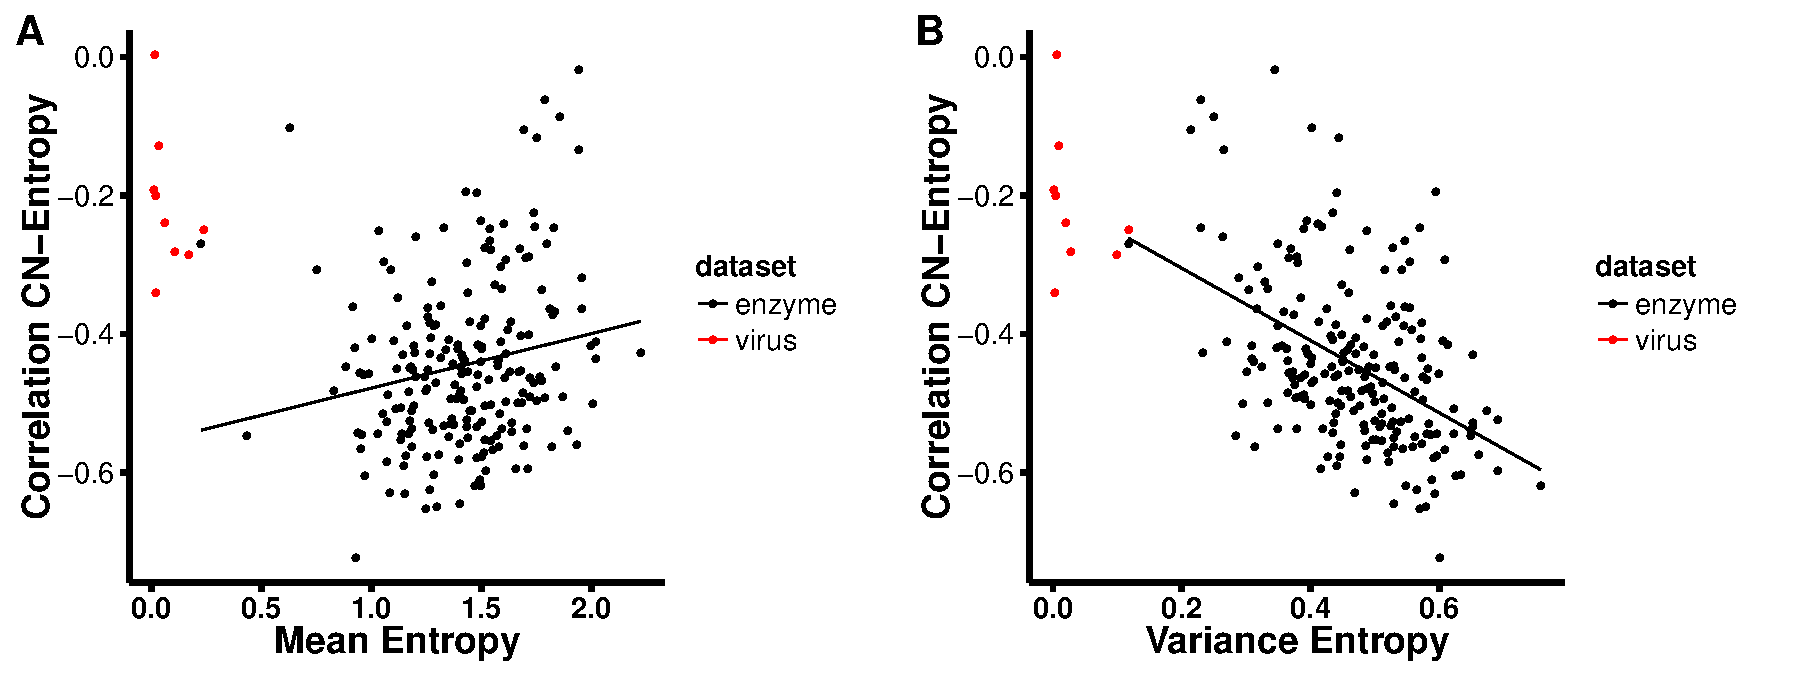
\includegraphics[width=7.5in]{entropy_cn_cor.pdf}}     
            \caption{Correlations between Contact Number (CN) and Entropy. For each protein we calculate the Spearman Correlation coefficient between CN and entropy at each site within the protein. A) Comparison between the correlation coefficients and mean entropy of site in each protein. The line indicates a linear regression through the enzyme proteins with mean entropy as a single predictor of the spearman correlations. B) Comparison between correlation coefficients and the variance of entropy of each protein. The enzyme proteins are colored in black and the virus proteins are visualized in red. For both WCN and CN the viral proteins have lower mean entropy and variance of entropy. The line indicates a linear regression through the enzyme proteins with variance entropy as a single predictor of the spearman correlations. Proteins with a larger variance in site entropy among sites tend to smaller CN-Entropy correlations in magnitude. Note: The entropy values in \cite{Shahmoradietal2014} were scaled.}
            \label{fig:entropy_cn_cor}
    \end{figure}

    \begin{figure}[H]
            \centerline{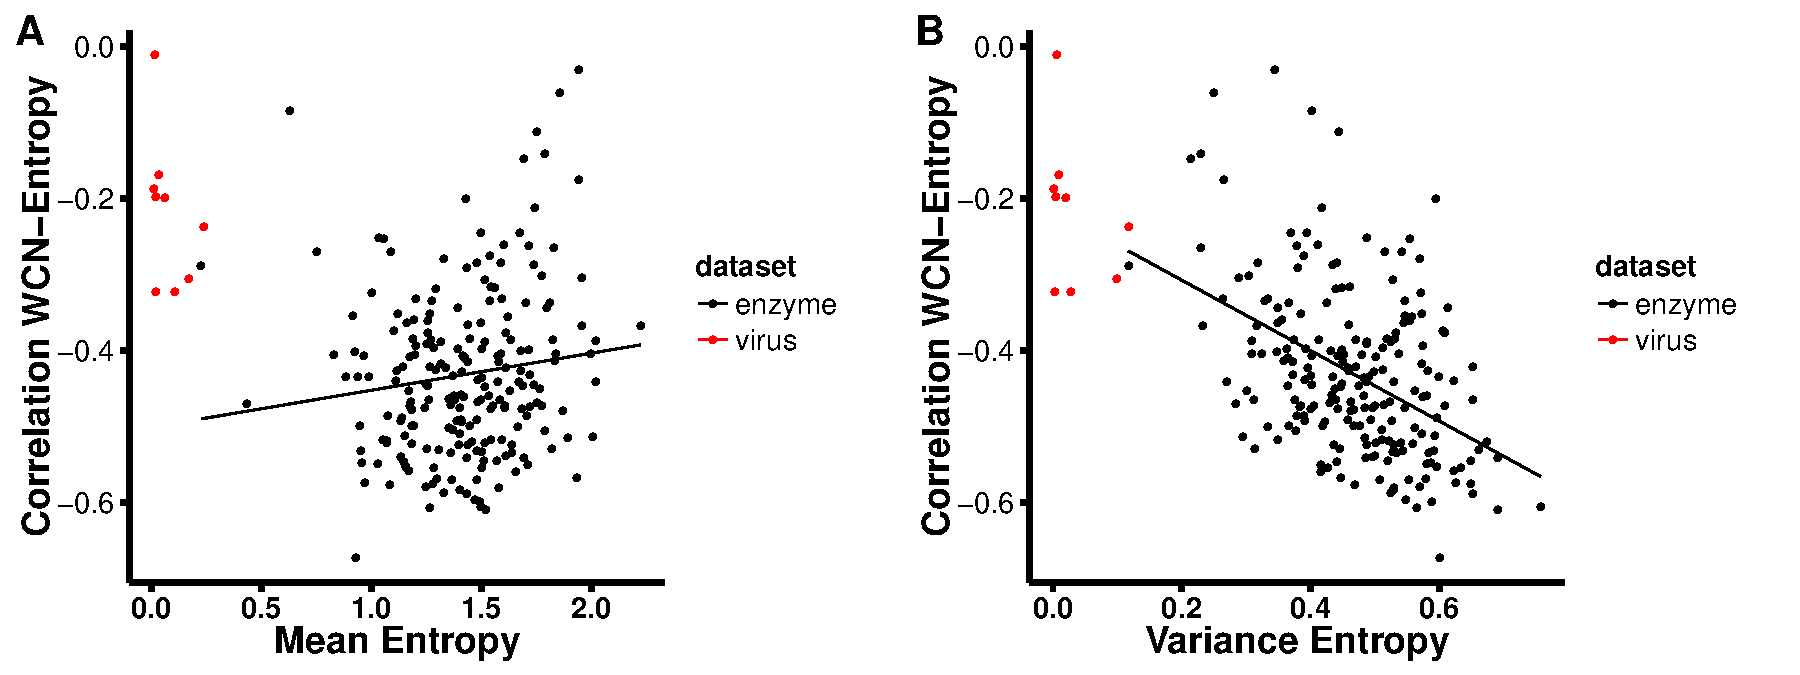
\includegraphics[width=7.5in]{entropy_wcn_cor.pdf}}     
            \caption{Correlations between Weighted Contact Number (WCN) and Entropy. A) Comparison between the correlation coefficients and mean entropy of site in each protein. B) Comparison between correlation coefficients and the variance of entropy of each protein. The enzyme proteins are colored in black and the virus proteins are visualized in red. Proteins with a larger variance in site entropy have smaller WCN-Entropy correlations in magnitude.}
            \label{fig:entropy_wcn_cor}
    \end{figure}

    \begin{figure}[H]
            \centerline{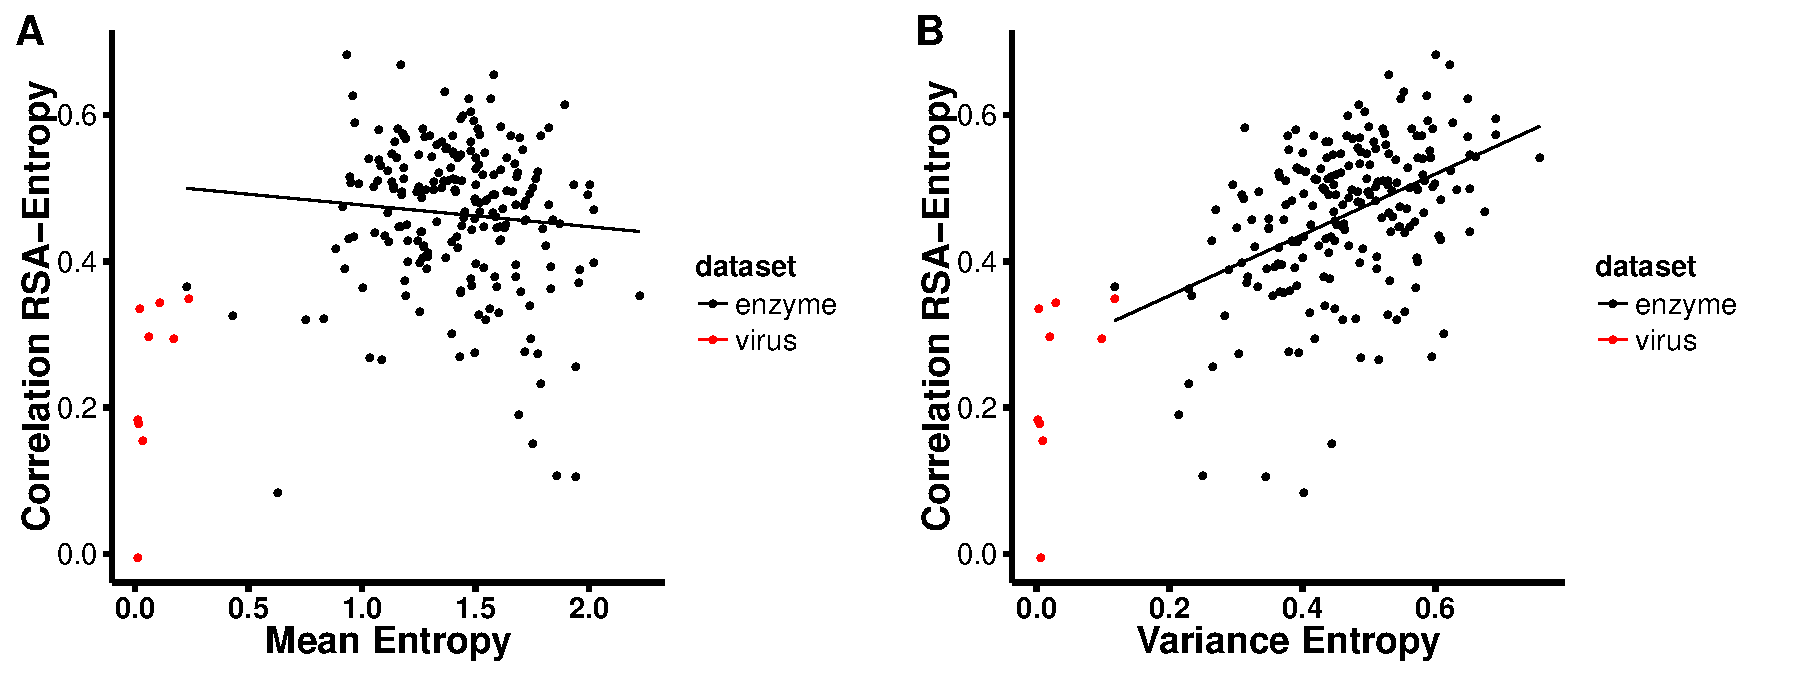
\includegraphics[width=7.5in]{entropy_rsa_cor.pdf}}     
            \caption{Correlations between Relative Solvent Accessibility (RSA) and Entropy. A) Comparison between the correlation coefficients and mean entropy of site in each protein. B) Comparison between correlation coefficients and the variance of entropy of each protein. The enzyme proteins are colored in black and the virus proteins are visualized in red. Proteins have a larger variance in site entropy have larger RSA-Entropy correlations.}
            \label{fig:entropy_rsa_cor}
    \end{figure}
        
        \begin{figure}[H]
            \centerline{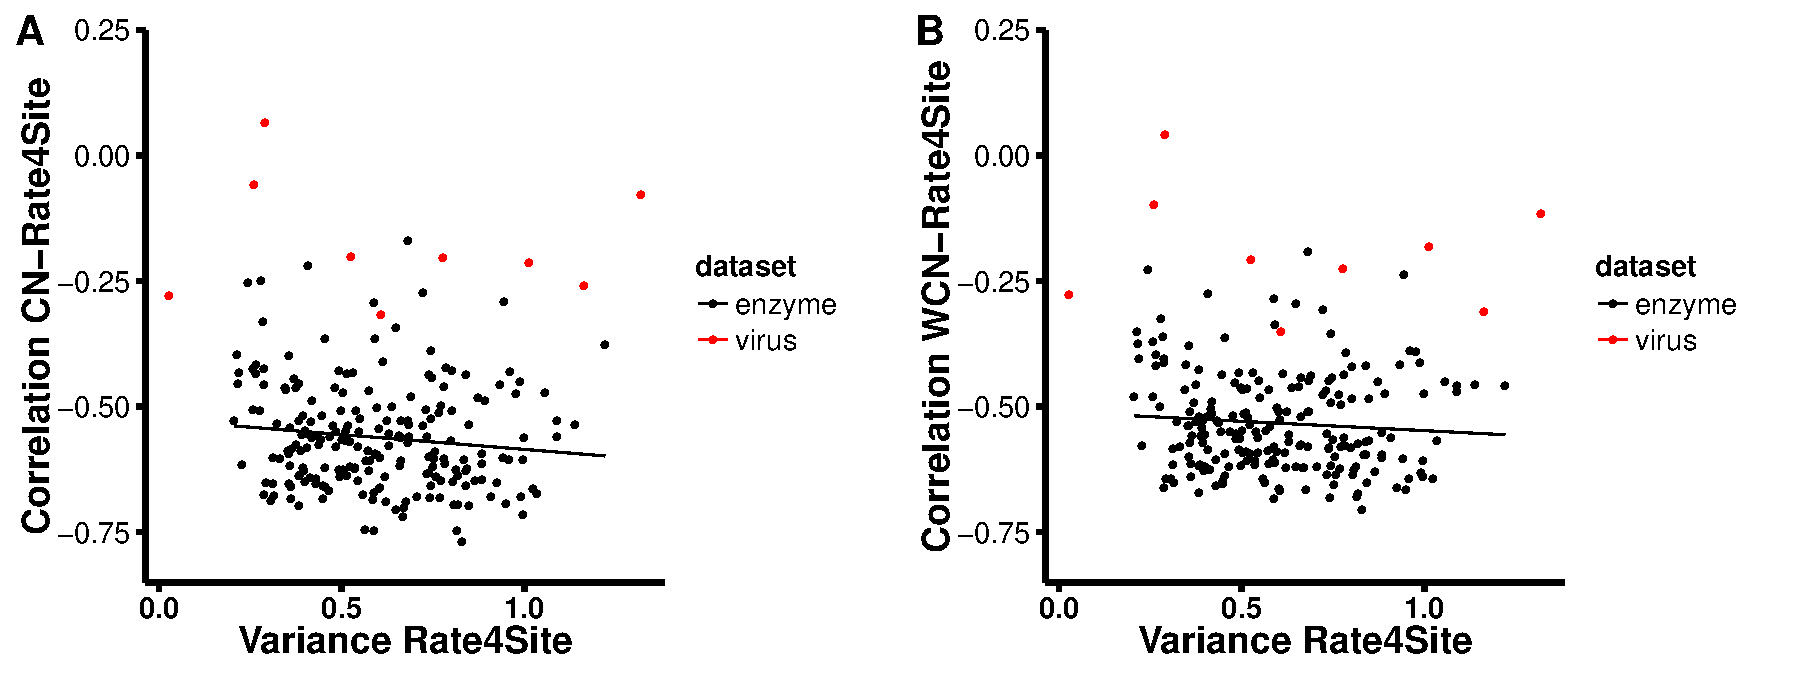
\includegraphics[width=7.5in]{rate_cor.pdf}}     
            \caption{Comparison of Rate4Site correlations and the variance of Rate4Site at sites. A) Comparison between the correlation coefficients between CN and Rate4Site and variance of Rate4Site of site in each protein. B) Comparison between correlation coefficients between WCN and Rate4Site and the variance of entropy of each protein. The enzyme proteins are colored in black and the virus proteins are visualized in red. There is no observable trend between the variance of evolutionary rate and the spearman correlations. }
            \label{fig:var_rate_cor}
    \end{figure}
        
            \begin{figure}[H]
            \centerline{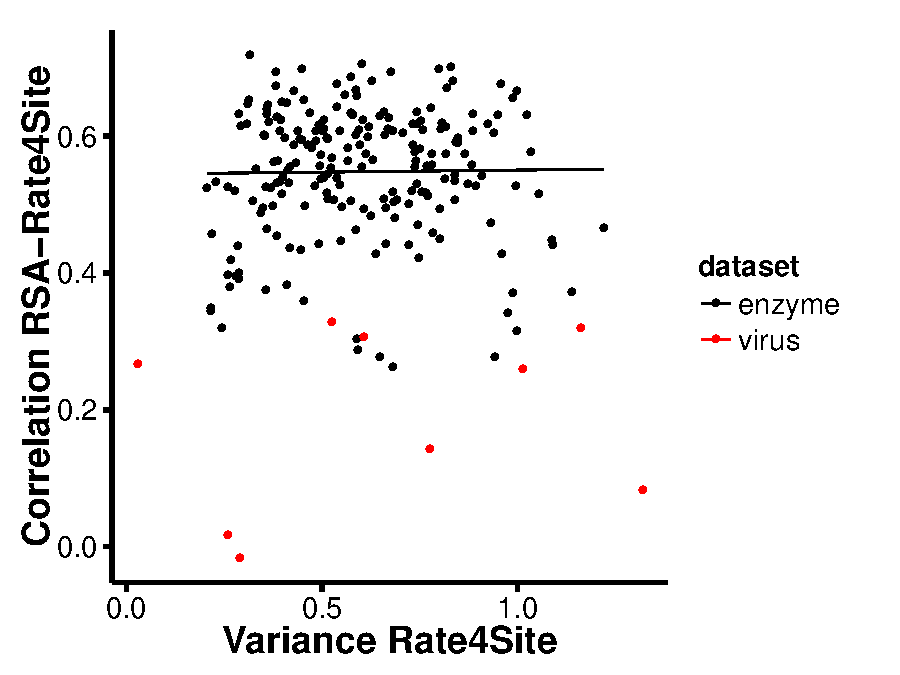
\includegraphics[width=4in]{var_rate_rsa_cor.pdf}}     
            \caption{Comparison of the correlations between RSA and Rate4Site and the variance of Rate4Site at sites. The enzyme proteins are colored in black and the virus proteins are visualized in red. The variance of evolutionary rate of a protein, as measured by Rate4Site, does not have a correlation with the spearman correlation between RSA and evolutionary rate for a given protein.}
            \label{fig:var_rate_rsa_cor}
    \end{figure}
    
%       \begin{figure}[H]
%            \centerline{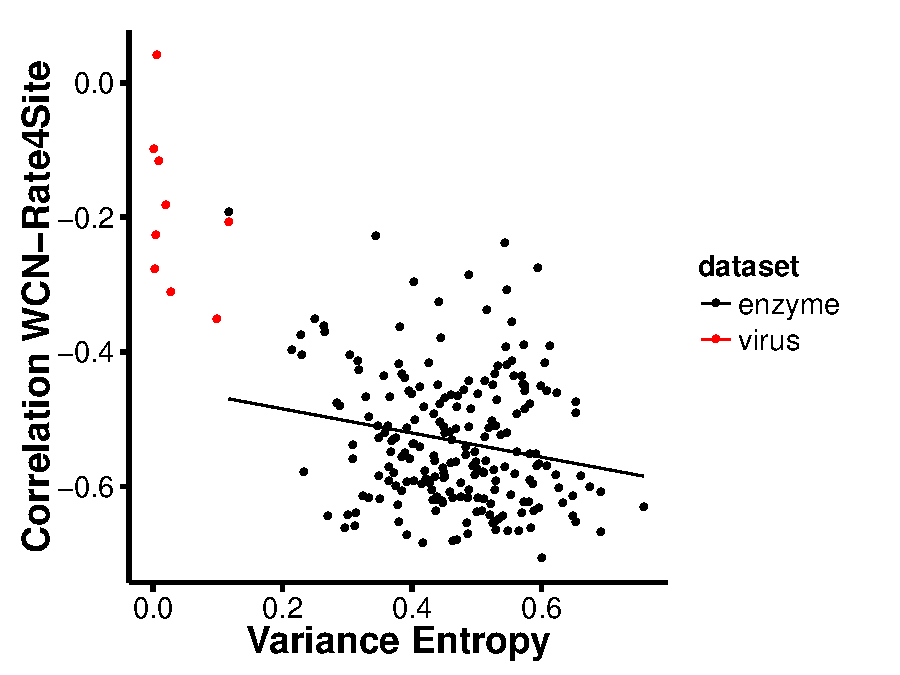
\includegraphics[width=5.0in]{var_entropy_rate_cor.pdf}}     
%            \caption{Relationship between WCN-Rate4Site correlations and the variance of entropy at sites. The enzyme proteins are colored in black and the virus proteins are colored red. }
%            \label{fig:var_entropy_rate_cor}
%    \end{figure}
 
 
        \begin{figure}[H]
            \centerline{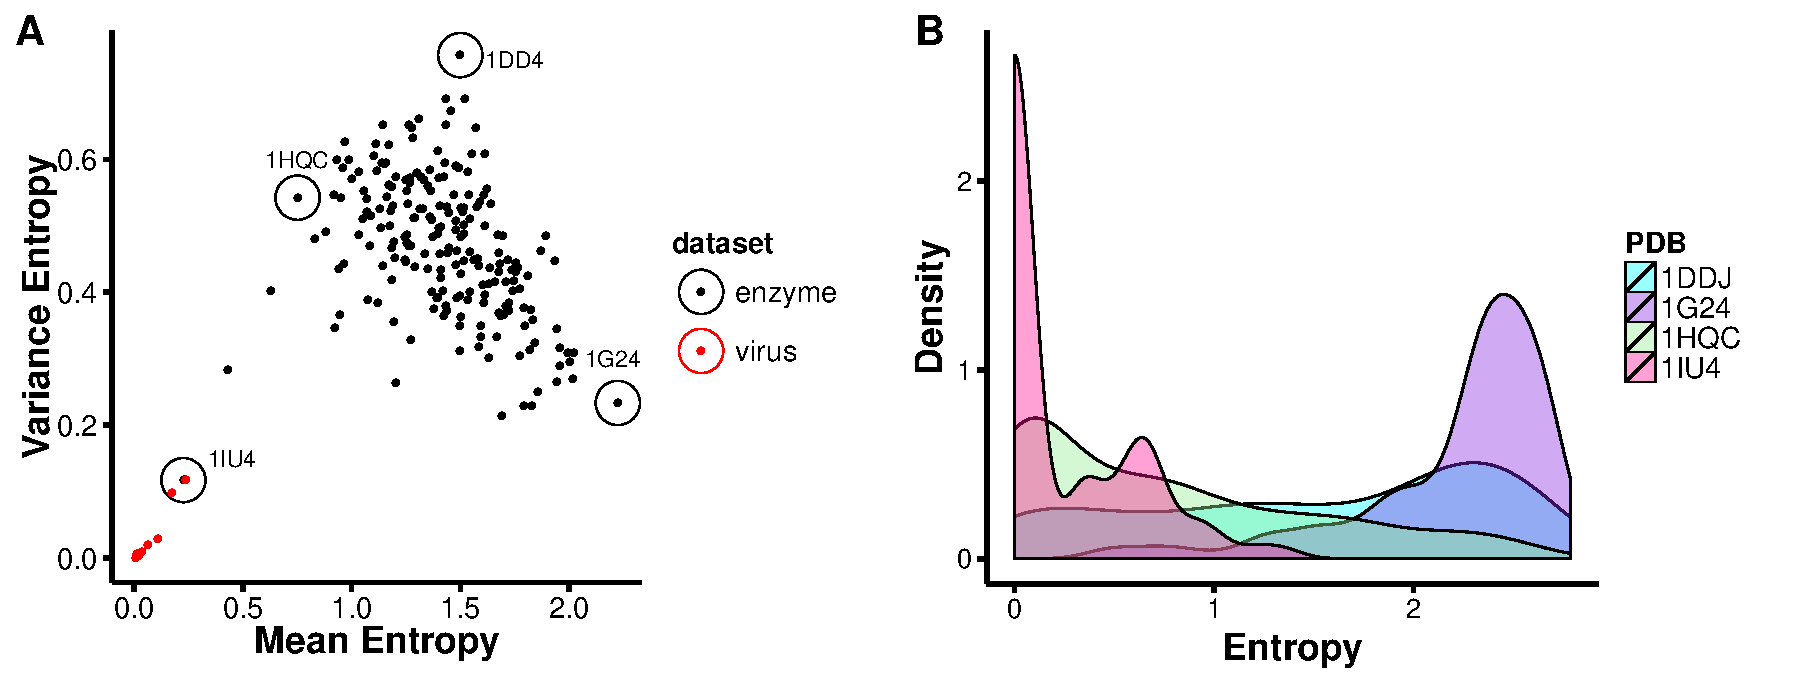
\includegraphics[width=6.5in]{protein_ex_plot.pdf}}     
            \caption{Comparison of the mean entropy and the variance of entropy for individual proteins. A)  Variance in entropy at sites compared against overall mean entropy for proteins. Four proteins of interest are highlighted by open circles. The enzyme proteins are colored in black and the virus proteins are colored red B-F) Distributions of site-wise entropy values for the five enzyme proteins highlighted in A. There are a variety of distributions in site entropy for different proteins.}
            \label{fig:protein_ex_plot}
    \end{figure}
     

\begin{center}
	\begin{table}[H]
	\begin{tabular}{| p{1.5cm} | p{2.5cm} | p{2cm} | p{2cm} | }
		\hline
		Dataset & Mean $\rho$ Entropy-CN  & Mean $\rho$ Entropy-WCN & Mean $\rho$ Entropy-RSA \\
		\hline	
		Enzyme &  $-0.445$  & $-0.432$ & $0.464$ \\[0.10cm]
	
		Virus & $-0.213$ & $-0.217$ & $0.237$ \\
		\hline	
	\end{tabular}
	\caption{Averages of the Spearman Correlation Coefficients between Structural Properties and Entropy. The structural properties analyzed are solvent accessibility as calculated by RSA and packing density as calculated by CN and WCN.}
	\label{table:entropy_stats}
	\end{table}
\end{center}

\begin{center}
	\begin{table}[H]
	\begin{tabular}{| p{1.5cm} | p{2.5cm} | p{2cm} | p{2cm} |  }
		\hline
		Dataset & Mean $\rho$ Rate4Site-CN  & Mean $\rho$ Rate4Site-WCN & Mean $\rho$ Rate4Site-RSA \\
		\hline	
		Enzyme &  $-0.445$  & $-0.432$ & $0.464$ \\[0.10cm]
	
		Virus & $-0.213$ & $-0.217$ & $0.237$ \\
		\hline	
	\end{tabular}
	\caption{Averages of the Spearman Correlation Coefficients between Structural Properties and Evolutionary Rate. Evolutionary rate is calculated with Rate4Site. The structural properties analyzed are solvent accessibility as calculated by RSA and packing density as calculated by CN and WCN.}
	\label{table:rate_stats}
	\end{table}
\end{center}

%Should I report the intercept%
\begin{center}
	\begin{table}[H]
	\begin{tabular}{ | p{5.0cm} | p{3cm} | p{3cm} | p{4cm} | }
	\hline
	Model & $\left \langle H \right \rangle$  & Dataset & Dataset*$\left \langle H \right \rangle$ \\	
	\hline
	$\rho  \text{\_CN--H}$   $ = $  $\left \langle H \right \rangle$ + Dataset + Dataset*$\left \langle H \right \rangle$ & $0.079 ^{**}$ & $0.382^{***}$  & $-0.583$   \\[1.2cm] 
		
	$\rho  \text{\_WCN--H}$  $ = $  $\left \langle H \right \rangle$ + Dataset + Dataset*$\left \langle H \right \rangle$& $0.049$ & $0.323^{***}$ & $-0.568$  \\[1.2cm] 	 
	 
	$\rho  \text{\_RSA--H}$  $ = $ $\left \langle H \right \rangle$ + Dataset + Dataset*$\left \langle H \right \rangle$ &  $-0.030$ & $-0.336^{***}$ & $0.903^{*}$ \\[1.2cm]

	$\rho  \text{\_CN--H}$   $ = $  $\left \langle H \right \rangle$ + Dataset + Dataset*$\left \langle H \right \rangle$ & $0.077^{**}$ & $0.336^{***}$  & NA  \\[1.2cm] 
		
	$\rho  \text{\_WCN--H}$  $ = $  $\left \langle H \right \rangle$ + Dataset + Dataset*$\left \langle H \right \rangle$& $ 0.047$ & $0.278^{***}$ & NA  \\[1.2cm] 	 
	 
	$\rho  \text{\_RSA--H}$  $ = $ $\left \langle H \right \rangle$ + Dataset + Dataset*$\left \langle H \right \rangle$ &  $-0.027$ & $ -0.264^{***}$ & NA \\
		
	
	
	
	\hline
	\end{tabular}
	\caption{Linear models predicting structural correlations with various quantities. Coefficient x represents the coefficient of the first predictor, coefficient y is the coefficient of the second predictor and coefficient z is the coefficient of the third predictor in each model.  *** means the p-value is less than 0.001. ** means the p-value is less than 0.01.  * means the p-value is less than 0.05. }
	\label{table:model_stats}
	\end{table}
\end{center}

\begin{center}
	\begin{table}[H]
	\begin{tabular}{ | p{5.0cm} | p{3cm} | p{3cm} | p{4cm} | }
	\hline
	Model & Variance H  & Dataset & Dataset*Variance H \\	
	\hline
	$\rho  \text{\_CN--H}$ $ = $ Variance H + Dataset + Dataset*Variance H & $-0.522^{***}$ &  $0.013$ & $-0.265$ \\[1.3cm] 	
	
	$\rho  \text{\_WCN--H}$ $ = $ Variance H + Dataset + Dataset*Variance H& $-0.464^{***}$ &  $0.023$ & $-0.325$ \\ [1.3cm] 	
	
	$\rho  \text{\_RSA--H}$ $ = $ Variance H + Dataset + Dataset*Variance H & $0.415^{***}$ & $-0.076$ & $0.927$ \\	
	
		$\rho  \text{\_CN--H}$ $ = $ Variance H + Dataset + Dataset*Variance H & $-0.524^{***}$ &  $0.004$ & NA \\[1.3cm] 	
	
	$\rho  \text{\_WCN--H}$ $ = $ Variance H + Dataset + Dataset*Variance H& $-0.466 ^{***}$ &  $ 0.012$ & NA \\ [1.3cm] 	
	
	$\rho  \text{\_RSA--H}$ $ = $ Variance H + Dataset + Dataset*Variance H & $0.422^{***}$ & $-0.044$ & NA \\	
	
	
	\hline
	\end{tabular}
	\caption{Linear models predicting structural correlations with various quantities. Coefficient x represents the coefficient of the first predictor, coefficient y is the coefficient of the second predictor and coefficient z is the coefficient of the third predictor in each model.  *** means the p-value is less than 0.001. ** means the p-value is less than 0.01.  * means the p-value is less than 0.05. }
	\label{table:model_stats}
	\end{table}
\end{center}

Make a table of the mean correlations and variance from both papers. 


\end{document}

